
\documentclass[a4paper, 12pt]{article}
\usepackage{a4wide}
\usepackage {amsmath}
\usepackage{amssymb}
\usepackage {graphicx}
\usepackage[utf8]{inputenc} 
\usepackage[francais]{babel}
\usepackage{fancyhdr}
\usepackage{setspace}
\usepackage{fancyhdr}
\usepackage{lastpage}
\usepackage{extramarks}
\usepackage{chngpage}
\usepackage{soul}
\usepackage{algorithmicx} 
\usepackage{algpseudocode} 
\usepackage{multicol}
\usepackage[usenames,dvipsnames]{color}
\usepackage{graphicx,float,wrapfig}
\usepackage{ifthen}
\usepackage{listings}
\usepackage{courier}
\usepackage{esint}
\usepackage{bbm}
\usepackage{graphics}
\usepackage{graphicx}
\usepackage{subfig}
\usepackage{epsfig}
\usepackage{pgf,tikz}
\usetikzlibrary{arrows}
\usepackage{braket}
\usepackage{MnSymbol,wasysym}
\usepackage{marvosym}
\usepackage{dsfont}
\usepackage{stmaryrd}

\lhead{} 
\chead{} 
\rhead{\bfseries Modes propres en Python} 
\lfoot{J.-C. Toussaint}
%\cfoot{} 
%\rfoot{\thepage}

% This is the color used for MATLAB comments below
\definecolor{MyDarkGreen}{rgb}{0.0,0.4,0.0}

% For faster processing, load Matlab syntax for listings
\lstloadlanguages{Matlab}%
\lstset{language=Matlab,                        % Use MATLAB
        frame=single,                           % Single frame around code
        basicstyle=\small\ttfamily,             % Use small true type font
        keywordstyle=[1]\color{Blue}\bf,        % MATLAB functions bold and blue
        keywordstyle=[2]\color{Purple},         % MATLAB function arguments purple
        keywordstyle=[3]\color{Blue}\underbar,  % User functions underlined and blue
        identifierstyle=,                       % Nothing special about identifiers
                                                % Comments small dark green courier
        commentstyle=\usefont{T1}{pcr}{m}{sl}\color{MyDarkGreen}\small,
        stringstyle=\color{Purple},             % Strings are purple
        showstringspaces=false,                 % Don't put marks in string spaces
        tabsize=5,                              % 5 spaces per tab
        %
        %%% Put standard MATLAB functions not included in the default
        %%% language here
        morekeywords={xlim,ylim,var,alpha,factorial,poissrnd,normpdf,normcdf},
        %
        %%% Put MATLAB function parameters here
        morekeywords=[2]{on, off, interp},
        %
        %%% Put user defined functions here
        morekeywords=[3]{FindESS, homework_example},
        %
        morecomment=[l][\color{Blue}]{...},     % Line continuation (...) like blue comment
        numbers=left,                           % Line numbers on left
        firstnumber=1,                          % Line numbers start with line 1
        numberstyle=\tiny\color{Blue},          % Line numbers are blue
        stepnumber=5                            % Line numbers go in steps of 5
        }

% Includes a MATLAB script.
% The first parameter is the label, which also is the name of the script
%   without the .m.
% The second parameter is the optional caption.
\newcommand{\matlabscript}[2]
  {\begin{itemize}\item[]\lstinputlisting[caption=#2,label=#1]{#1.m}\end{itemize}}

\pagestyle{fancy}

\begin{document}

\bibliographystyle{alpha}

\title{Modes propres de vibration}

%\author{
%\texttt{jean-christophe.toussaint@phelma.grenoble-inp.fr}
%}
\date{\today}
%\date{\vspace{-10ex}}
 
\maketitle

%\vspace{1cm}

\section{Modes propres associés à une assemblée de ressorts}


Le but de cette étude est de calculer les fréquences propres et les modes propres d'un oscillateur
linéaire formé de  quatre sphères  couplées deux à deux par des ressorts. 

Pour simplifier, on suppose que les sphères sont de masse identique $m$ et que les  ressorts
ont tous la même constante de  raideur $k$.   

\begin{figure}[!h]
\centering
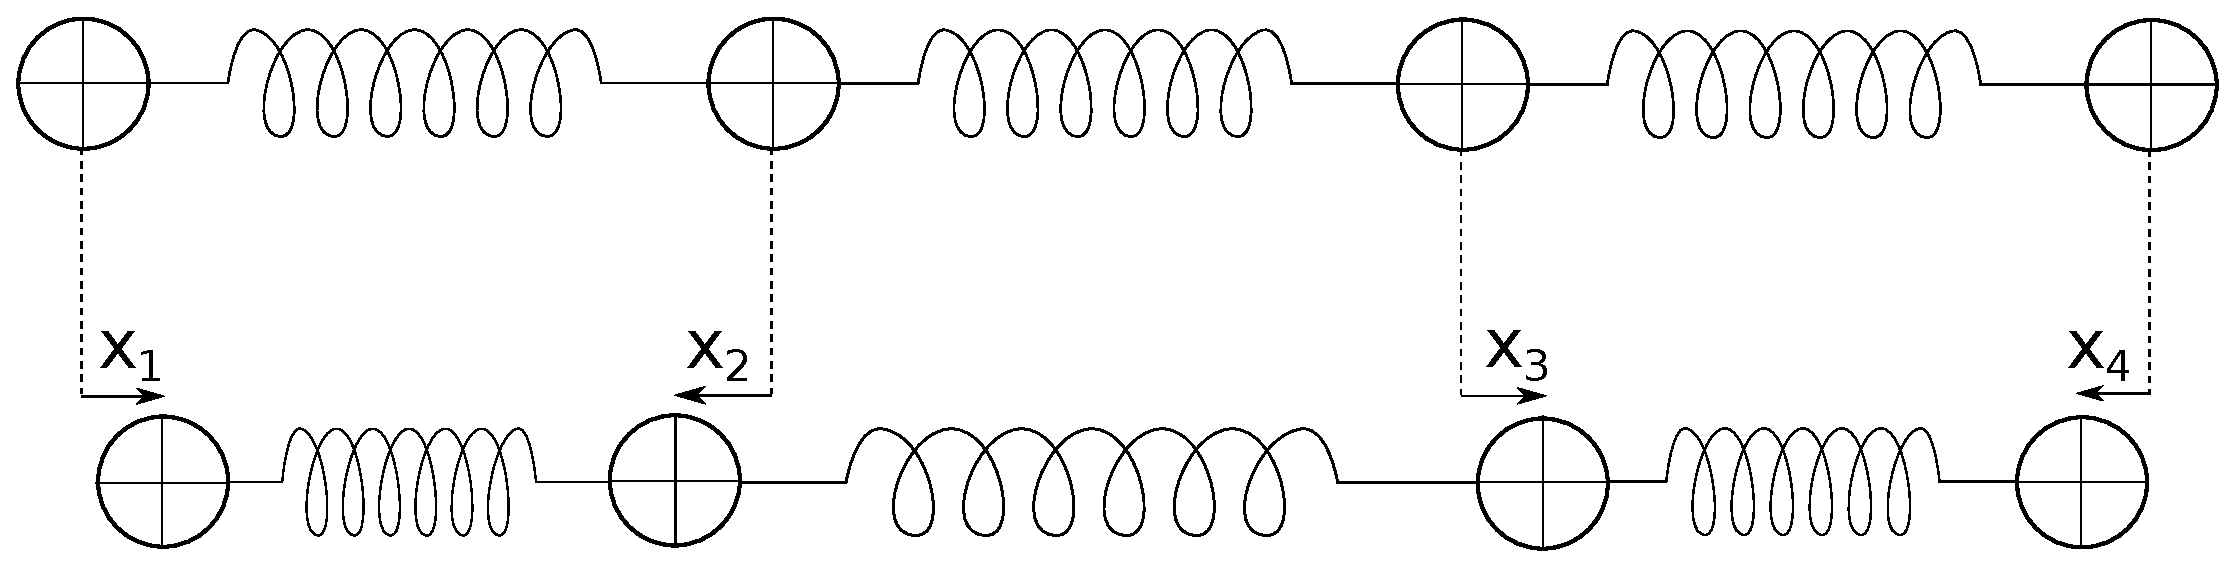
\includegraphics[scale=0.4]{spring4m.eps}
\caption{ressorts couplés}
\label{Res}
\end{figure}


Le principe fondamental de la dynamique appliqué successivement à chaque masse mène à un système
de quatre équations différentielles couplées:

$$
\left \{
\begin{array}{r c l}
m \ddot x_1 &=& -k \, (x_1-x_2)  \\
m \ddot x_2 &=& -k \, (x_2-x_1)  -k \, (x_2-x_3) \\
m \ddot x_3  &=&  -k \,(x_3-x_2) -k \,(x_3-x_4)\\
m \ddot x_4 &=& -k \, (x_4-x_3)  
\end{array}
\right .
\Longleftrightarrow
\left(
\begin{array}{c}
 \ddot x_1 \\  \ddot x_2 \\  \ddot x_3 \\  \ddot x_4
\end{array}
\right) = - {k \over m}
\left(
\begin{array}{rrrr}
1   & -1 & 0  & 0  \\
-1  & 2 & -1 & 0 \\
0  & -1 & 2 & -1 \\
0  & 0 & -1 & 1 \\
\end{array}
\right)
\left(
\begin{array}{c}
x_1 \\ x_2 \\ x_3 \\ x_4
\end{array}
\right)
$$

En se plaçant dans le régime harmonique et en utilisant
la notation complexe, on écrit : $x_i(t)=a_i \, exp(i\omega t)$ où $i \in [1, 4]$ et $a_i \in \mathbbm{C}$.
Noter que les déplacements physiques coïncident avec les parties réelles de ces quantités.\\

On obtient, en notant ${\omega_0^2}=k/m$, le système linéaire suivant:
$$
{\omega_0^2}
\left(
\begin{array}{rrrr}
1   & -1 & 0  & 0  \\
-1  & 2 & -1 & 0 \\
0  & -1 & 2 & -1 \\
0  & 0 & -1 & 1 \\
\end{array}
\right)
\left(
\begin{array}{c}
a_1 \\ a_2 \\ a_3 \\ a_4
\end{array}
\right)=
{\omega^2}
\left(
\begin{array}{c}
a_1 \\ a_2 \\ a_3 \\ a_4
\end{array}
\right) 
$$

Le problème revient à diagonaliser une matrice de couplage que l'on note $K$. 
$$
K=
{\omega_0^2}
\left(
\begin{array}{rrrr}
1   & -1 & 0  & 0  \\
-1  & 2 & -1 & 0 \\
0  & -1 & 2 & -1 \\
0  & 0 & -1 & 1 \\
\end{array}
\right)
$$
où chaque valeur propre  $\lambda$ correspond au carré de la pulsation propre ${\omega}$.

\subsection{Mise en application}

Développer un script Python permettant de calculer les pulsations propres ainsi que les modes associés.
{\it Remarque : en Python, l’indexation des tableaux commence à 0.}

\begin{itemize}
\item La matrice $K$ est une matrice pleine stockée dans un tableau numpy.ndarray.
Les valeurs propres et vecteurs propres sont calculées avec la fonction {\tt linalg.eig} de la librairie {\tt numpy}.
\item La matrice $K$ est une matrice creuse.
On utilisera la fonction {\tt sparse.csr\_matrix} pour stocker les termes non nuls de la
librairie {\tt scipy}.
Les valeurs propres et vecteurs propres sont calculées avec la fonction {\tt sparse.linalg.eigsh} de la librairie {\tt scipy}.
\end{itemize}



\section{Application de conditions de déplacement nul en certains noeuds}

On présente ici une méthode générale pour calculer les modes propres en s'appuyant sur
l'étude précédente lorsque certaines masses du systèmes sont fixes.
Ces conditions s'apparentent aux conditions de dirichlet du type $x_i=0$.

En notant $N_d$ le nombre de masses où  la condition de dirichlet est imposée, 
le nombre de degrés de liberté se réduit alors à $N_{dof}=N-N_d$ et correspond 
ici au nombre de masses pouvant osciller.\\

\subsection{Algorithme}
L'algorithme consiste à former une liste $l$ où le numéro de chaque masse pouvant osciller,
apparaît de façon unique. Sa
taille est $N_{dof}=N-N_d$ et s'identifie, ici,  au nombre de degrés de liberté. \\

On forme ensuite une matrice de projection $P$ permettant de passer de l'espace des solutions à $N$ degrés de 
liberté (étude précédente) à celui restreint à $N_{dof}$ degrés de liberté.
Les dimensions de P sont $N_{dof} \times N$ (nombre de lignes $\times$ nombre de colonnes).
On initialise d'abord la matrice $P$ à zéro;
puis en parcourant séquentiellement la liste $l$, on impose $P[i, l[i]]=1$ avec $\llbracket 0, N_{dof}-1  \rrbracket$.
On remarque que $P P^t = {\tt Id}(N_{dof})$ .\\

Une autre façon de construire la matrice $P$ est de l'initialiser avec  la matrice identité ${\tt Id}(N)$
puis de supprimer toutes les lignes correspondant aux noeuds de dirichlet. Cette technique
est bien adaptée à Numpy/Scipy en masquant les numéros de lignes correspondant aux noeuds de dirichlet.


\begin{lstlisting}[language=Python]
def delete_rows(mat, indices):
    indices = list(indices) # transformation en liste
    mask = np.ones(mat.shape[0], dtype=bool) # ligne de True
    mask[indices] = False # True->False pour les noeuds de dirichlet
    return mat[mask]
\end{lstlisting}

\begin{figure}[!h]
\centering
\includegraphics[scale=0.25]{matP.eps}
\caption{exemple de matrice $P$ avec $ld=[0, 2]$}
\label{matP}
\end{figure}

On construit ensuite $K_p$ qui est la matrice projetée de $K$ dans l'espace
solution à $N_ {dof}$ degrés de liberté: $K_p=P K P^t$ .
C'est cette matrice qui est finalement diagonalisée. On obtient alors les valeurs propres $\lambda_p$ associées
aux vecteurs propres $a_p$. Autrement dit, cela revient à résoudre:
$P K P^t a_p= \lambda_p a_p$.

On reconstruit la solution dans l'espace à $N$ corps en appliquant $a=P^t a_p$. 
Elle vérifie automatiquement, $a[i]=0$ pour tout noeud $i$ de dirichlet.

\subsection{Mise en application}

$\bullet$ Utiliser sous Numpy, la fonction {\tt ld=numpy.unique(ld)} pour éliminer tout doublon dans la liste {\tt ld}.

$\bullet$ Calculer numériquement les modes propres du système lorsque les masses $0$ et $2$ sont fixes.

$\bullet$ Vérifier vos résultats numériques avec une approche analytique.


\section{Modes propres d'une corde}

Le but de l'exercice est de caractériser les modes de vibration $u_k(x)$ selon Oz d'une corde. 
Dans la limite des faibles amplitudes de vibration, 
ils sont solutions de l'équation d'Helmholtz stationnaire :

\begin{equation}
\partial_x^2 \; u_k + k^2 \; u_k=0
\label{Helm}
\end{equation}

On considère que la corde est fixée à ses extrémités.


\subsection{Partie Mathématique}

La corde de longueur $L_x$ est dicrétisée en différences finies
avec une grille comportant $N_x$ noeuds. On note $\Delta x$ et
le pas de la grille.

\begin{enumerate} 
 \item  On numérote de manière unique les noeuds dans $\llbracket 0, N_x-1  \rrbracket$. 
 L'abscisse d'un noeud est donnée par la relation : $x = ix*\Delta x$.
On en déduit que $\Delta x = L_x /(N_x-1)$.
    
 \item L'expression discrète en différences finies, de l'opérateur laplacien appliqué à $u(x)$ 
 en un point {\bf intérieur} $x$ de la grille est donnée par :

  \begin{equation}
 \partial_x^2 \; u_k (x)= \frac{ u_k(x+\Delta x)+ u_k(x-\Delta x)-2 u_k(x)}{\Delta x^2}
 +\vartheta(\Delta x)^2
\end{equation}

% \begin{equation}
% \partial_x^2 \; u_k (x)= \frac{1}{\Delta x^2}  u_k(x+\Delta x)+ 
% \frac{1}{\Delta x^2}  u_k(x-\Delta x)-2 \frac{1}{\Delta x^2}  u_k(x)
% +\vartheta(\Delta x)^2
%\end{equation}

\item L'équation  \eqref{Helm}  s'écrit après discrétisation, sous la forme matricielle suivante:
\begin{equation}
\sum_j K_{i, j} \; u_j = k^2 u_i = \lambda_k u_i
\label{HelmDis}
\end{equation}
Préciser la forme générale de la matrice K sans se soucier des bords.

\item On tient maintenant compte du déplacement nul des noeuds du bord.
Dans le cas d'une grille $4 \times 4$ de pas de maille $\Delta x$, donner
précisément le remplissage de $K$ avec l'expression des termes non-nuls. 
Dans la suite, on verra comment éliminer les degrés de liberté liés aux noeuds de dirichlet.
On admet que pour tout noeud ${i}$ du bord, on laisse vide la ligne  ${i}$ dans la matrice $K$.
Utiliser le patron de la matrice vide fournie ci-après.

\end{enumerate} 

\begin{center}
   \begin{tabular}{| c | c | c | c | c  |}
     \hline
        & 0  & 1 & 2 &  3  \\ \hline
     0 &     &    &    &      \\ \hline
     1 &     &    &    &      \\ \hline
     2 &     &    &    &      \\ \hline
     3 &     &    &    &      \\ \hline
   \end{tabular}
 \end{center}
 

%\subsection{Phase de programmation et de simulation}
  
\subsection{Mise en application}

On vous fournit un embryon de programme {\tt FD\_helm.py}  à compléter,
utilisant une structure de
données {\tt fdm} pour stocker tous les paramètres de la simulation.

\begin{enumerate} 

\item Compléter la fonction  {\tt \_\_dirichlet} permettant de construire la liste $ld$ 
des noeuds du bord où sont appliquées la conditions de dirichlet.
On rappelle que
l'instruction {\tt ld.append(e)} permet d'insérer l'élément e dans la liste ld. 
Utiliser sous Numpy, la fonction {\tt ld=numpy.unique(ld)} pour éliminer tout doublon dans la liste {\tt ld}.

% \matlabscript{founddir}{test dirichlet}

\item Compléter la fonction  {\tt \_\_build\_K} permettant de remplir la matrice $K$ pour une grille
de taille $N_x$.  On rappelle que toute ligne $n$ de $K$ correspondant à un noeud
de dirichlet n'est pas remplie. \\
Pour tester l'appartenance d'un noeud $n$ dans la liste {\tt ld}, on utilisera l'expression booléenne
 {\tt n in ld}. 

\item Compléter  la fonction  {\tt solve} permettant de calculer la $n^{eme}$ plus petite valeur propre
en module ainsi que le mode propre associé. On utilisera la fonction Numpy {\tt eig} 

\item Pour un système de taille $L_x=2m$, déterminer les 4 premiers modes de basse énergie et comparer à la solution analytique en $\sin(k_x x)$ de l'équation d'Helmholtz \eqref{Helm}. 
Reporter les valeurs propres et les contours des modes associés.

\end{enumerate} 

% \matlabscript{FDhelmM1etud}{Embryon de programme}
\end{document}

